\section{Vortex formation at planetary gap edges in layered
  discs}\label{disc-planet} 
The previous simulations, while necessary to isolate the effect of 
viscosity on the linear RWI, has the disadvantage that the radially
structured viscosity profile may act to source radial disc structure
in the non-linear regime. In this section, we employ a radially smooth
viscosity profile and use 
disc-planet interaction to
create the disc structure required for instability. We therefore expect viscosity to only
act as a damping mechanism. 

Vortex formation at gap edges is seen in many  
2D and 3D hydrdynamical simulations of giant planets in low viscosity discs 
\citep{valborro07,lin10,lin11a,lin12}. The fact that this is due to
the RWI has been explicitly verified through linear stability
analysis of planetary gap profiles produced from 2D simulations
\citep{valborro07,lin10}. Here, we simulate gap-opening giant planets
in 3D discs where the kinematic viscosity varies with height above the
disc midplane. Our numerical experiments are similar in spirit to
those performed by \cite{pierens10}, but our focus here is gap
stability in a layered disc. 
 
\subsection{Radially smooth viscosity profile for disc-planet
  interaction}\label{planet_visc_mode} 
Using the same notation as \S\ref{visc_model}, we impose a viscosity
profile $\hat{\nu}$ such that 
\begin{align}\label{planet_visc_profile}
  \hat{\nu}\Sigma_i(R)=
  \hat{\nu}_0\left[1+Q(\psi)\right]\Sigma_i(r_0)   
\end{align}
We have set the dimensionless argument in Eq. \ref{step} to
$\zeta=\psi$. Recall $\psi=\pi/2-\theta$ is the angular height away from the midplane. 
The viscosity increases from its floor value $\hat{\nu}_0$ by a factor
$A_\nu$ for $\psi > \zeta_\nu$. So the viscous layer is 
a wedge in the meridional plane, which conveniently fits into our
spherical grid. We set the floor viscosity $\hat{\nu}_0=2.5\times 10^{-7}$. 
The angluar thickness of the viscosity transition is fixed to $\Delta\zeta_\nu =
0.2h$. Fig. \ref{planet_visc2d} gives an example of this 
viscosity profile. %We will quote the thickness of the viscous layer as a 
%percentage of the entire $\theta$ domain size. 

\begin{figure}
  \centering
  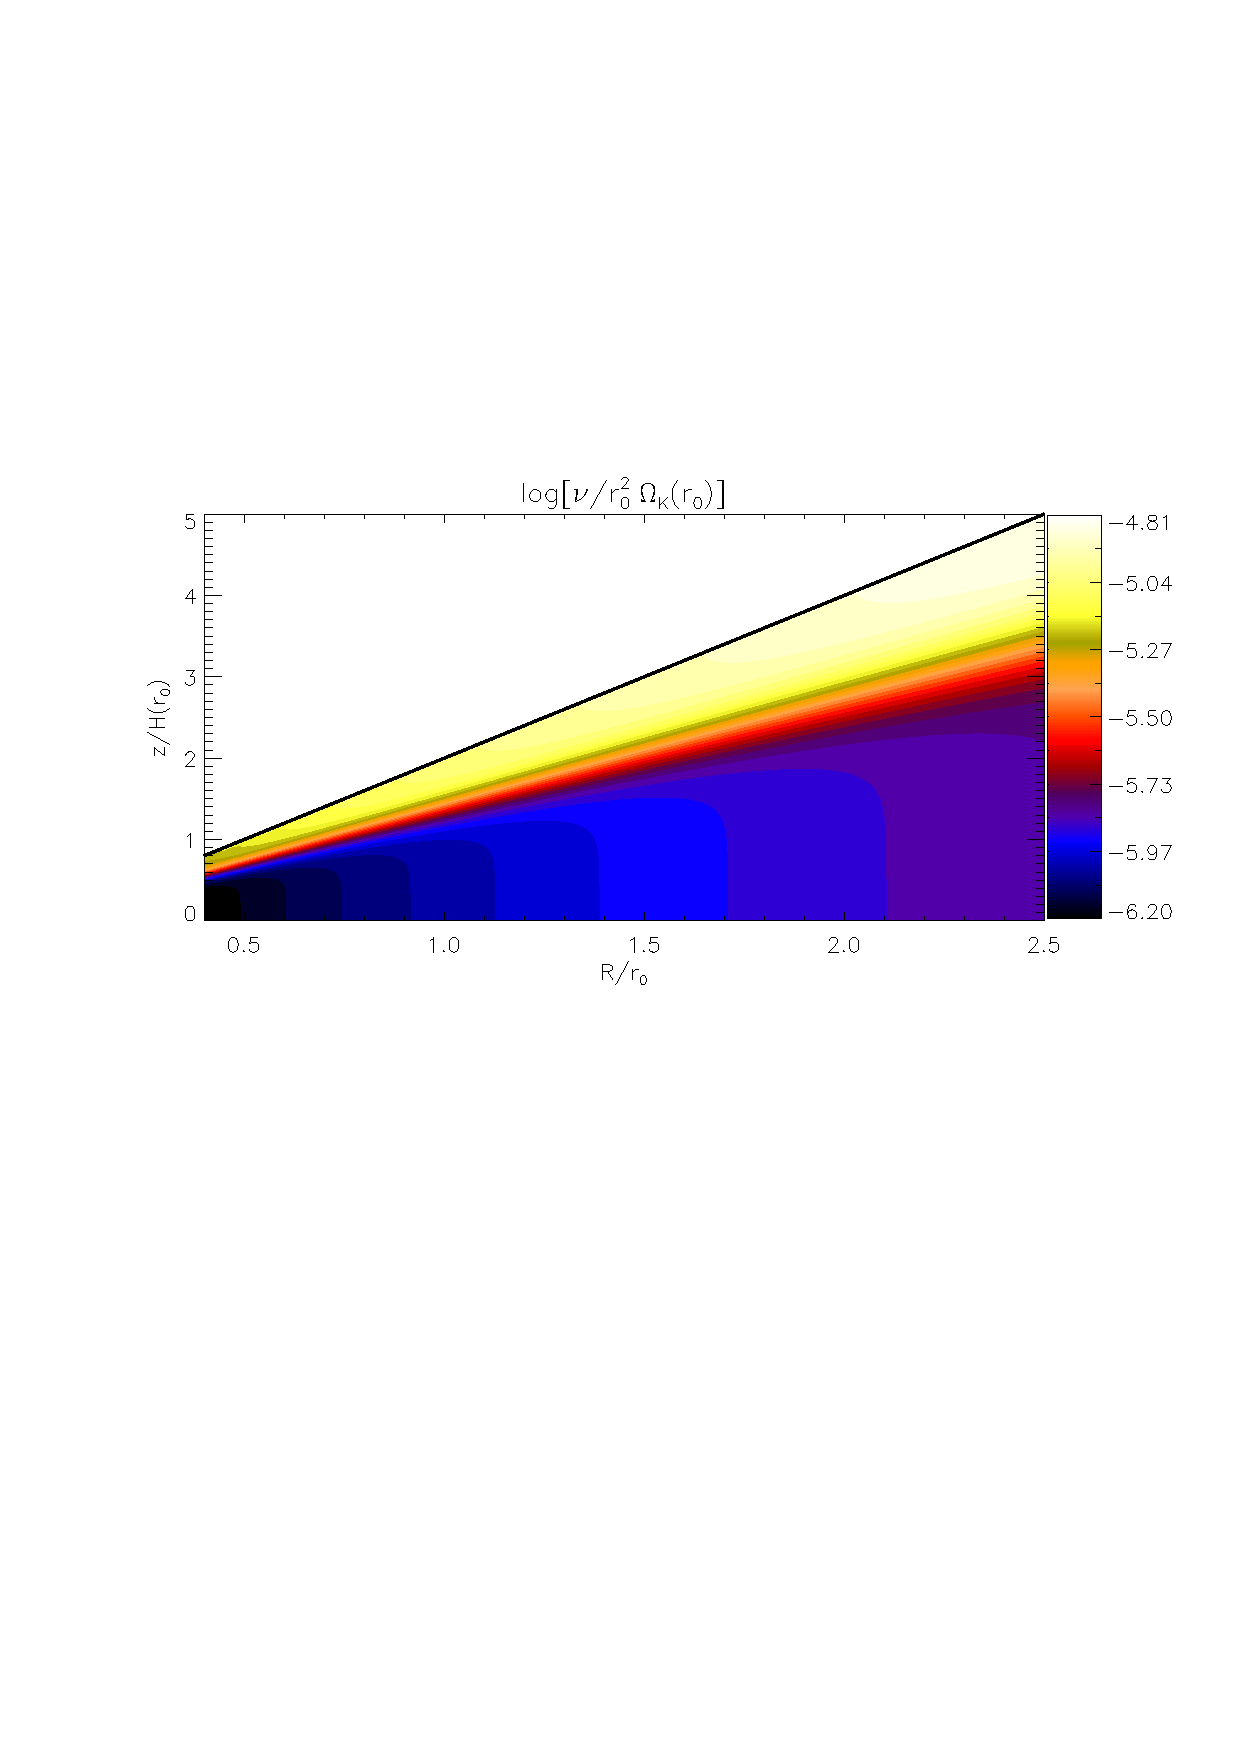
\includegraphics[width=\linewidth]{figures/pdisk_visc2d_planet}
  \caption{Example of the `wedge' viscosity profile
    imposed in disc-planet simulations
    (Eq. \ref{planet_visc_profile}).  
    For a disc with constant aspect ratio, as chosen here, the viscous
    layer occupies a constant number of scale heights across the
    radial range. This specific plot corresponds to case P1, so the
    viscous layer (yellow-white colours) always occupies the uppermost
    $H$ at each cylindrical radius. 
    The solid line
    delineates the upper boundary of the computational domain.
    \label{planet_visc2d}}
\end{figure}

\subsection{Disc-planet simulations} 
We simulate locally isothermal discs with constant aspect-ratio
$h=0.05$ (by choosing $q=1$), vertical extent $n_h=3$ scale-heights 
and radial extent $[\rin,\rout]=[0.4,2.5]r_0$. Initially the surface density is smooth
($A=1$) with zero meridional velocity ($v_r=v_\theta=0$). 
%cylindrical radial velocity is given by
%Eq. \ref{init_vr}. 
The standard resolution is $(N_r, N_\theta,
N_\phi)=(256, 32n_h, 768)$, corresponding to $6,\,32,\,6$ 
cells per $H$ along the $r,\theta,\phi$ directions at the reference
radius. We apply a damping rate $\hat{\gamma}=2$ with the reference
velocity field $\bm{v}_\mathrm{ref}=(0,0,v_\phi)$ in spherical
co-ordinates.   

We insert into the disc a planet of mass  
$M_p=10^{-3}M_*$, which corresponds to a Jupiter mass planet if
$M_*=M_{\sun}$. The softening length adopted for the planet potential is
$\epsilon_p=0.5r_h$. The planet potential is switched on 
smoothly over $t\in[0,10]P_0$. We note that the disc can be considered
as two-dimensional for gap-opening giant planets, because the Hill
radius $r_h$ exceeds the local scale-height $H_0$ ($r_h/H_0\simeq1.4$
in our cases).   

We remark that the above choice of physical and numerical parameter
values are typical for global disc-planet simulations
\citep[e.g.][]{valborro06,mignone12}.   


\subsubsection{Runs} 
The fiducial case P0 has $A_\nu=1$ so there is no viscous layer, thus
$\hat{\nu}\sim 10^{-7}$ ($\alpha\sim 10^{-4}$) everywhere. Vortex
formation is then expected because the typical viscosity
value adopted for disc-planet simulations, $\hat{\nu}\sim 10^{-5}$ or
$\alpha\sim 10^{-3}$, is known to surpress vortex formation in 2D
\citep{valborro07, mudryk09}. 
For case P0.5 and P1 we set $A_\nu=100$ with transition angle $\zeta_\nu=2.5h$ and
$2h$, respectively. Thus the viscous layer with $\hat{\nu}\sim10^{-5}$
($\alpha\sim10^{-2}$) occupies the uppermost $0.5H$ and $H$ of the vertical
domain. %vortex formation is not expected to occur for such high
        %viscosity values. 
We also consider case P0R, in which we restart case P0 from 
$t=100P_0$ but with the layered viscosity profile of case P1. 

%also have additional runs for testing. these use n_h=2 for speed

%%%%%%%%%%%%%%%%%%%%%%%%%%%%%%%%%%%%%%%%%%%%%%%%%%%%%%%%%%%%%%%%%%%%%%%%%%%%%%%


\subsection{Results}
Table \ref{planet_sims} summarises the disc-planet simulations. 
We focus on vortex-formation at the outer gap edge. 
The non-axisymmetric mode amplitude in the last column was 
averaged over the shell $r\in[1.3,1.6]r_0$ and over time 
$t\in[150,200]P_0$. 
%We examine the $m=1$ mode since 
%for non-self-gravitating planetary gaps, if unstable, usually develop
%a single vortex in quasi-steady state \citep{valborro07,lin10}.   

%for  mode amp: spatial average over [1.2,1.6], time average over [100,150]P_0

\begin{table}
  \centering
  \caption{Summary of disc-planet simulations. These runs employ the
    `wedge' viscosity model described by
    Eq. \ref{planet_visc_profile}. The thickness of the viscous layer
    is measured from the upper disc boundary. Case P0.5 employs the
    viscosity profile of P0 for $t\leq100P_0$, and that of P1 for 
    $t>100P_0$.\label{planet_sims}}
    \begin{tabular}{lcccr}
      \hline\hline
      Case & $A_\nu$ &$\zeta_\nu/h$ & visc. layer& vortex \\ 
      \hline
      P0      &    1     &    $\infty$      & 0     &   YES    \\
      P0R    &    1$\to$100 & $\infty\to2.0$ &$0\to H$  & ?  \\
      P0.5    &    100 & 2.5 &$0.5H$ &  ?           \\ 
      P1      &    100   &    2.0      & $H$    &  NO    \\ 
%      P2      &    100   &    1.0      & $2H$  &         &\\ 
      \hline
  \end{tabular}
\end{table}

%density perturbation evolution. snapshots at t=50, 100, 150, 200. 
%azi averaged vortensity. t=50 and t=200
%kinetic energy. m=1 ke 
%additional experiments. case p0.5. strictly isothermal sims. 

%p0 and p1 show initial development m=4

Fig. \ref{jup0_3h} compares the time evolution of the midplane density
perturbation $\Delta\rho(z=0)$ for cases P0, P0.5 and P1. Note that in 
all cases the RWI with $m=4$ develops early on ($t\simeq20P_0$),
consistent with the limited effect of viscosity on the linear
instability, as found above. 

However, comparing case P0 and P1 shows that the non-linear evolution
is significantly affected by layered viscosity. Despite the fact that
the viscous layer only occupies $\sim4\%$ of the total column density
in case P1, its evolution diverges from case P0 from $t\simeq50P_0$.  


%Case P3 is essentially identical to case P0, so the 
%vortex instability is not affected by vertical domain size. We note
%that the viscosity is increased in the disc atmosphere, where the
%density is a factor $\sim 7$ times smaller than the midplane (but the
%viscosity is $100$ times larger). The viscous layer has surpressed
%vortex formation. This implies that vortex formation via
%the RWI at planetary gap edges can not tolerate a signigicantly
%viscous atmosphere, even if such a layer only occurs away from the
%midplane.    

\begin{figure*}
   \centering
   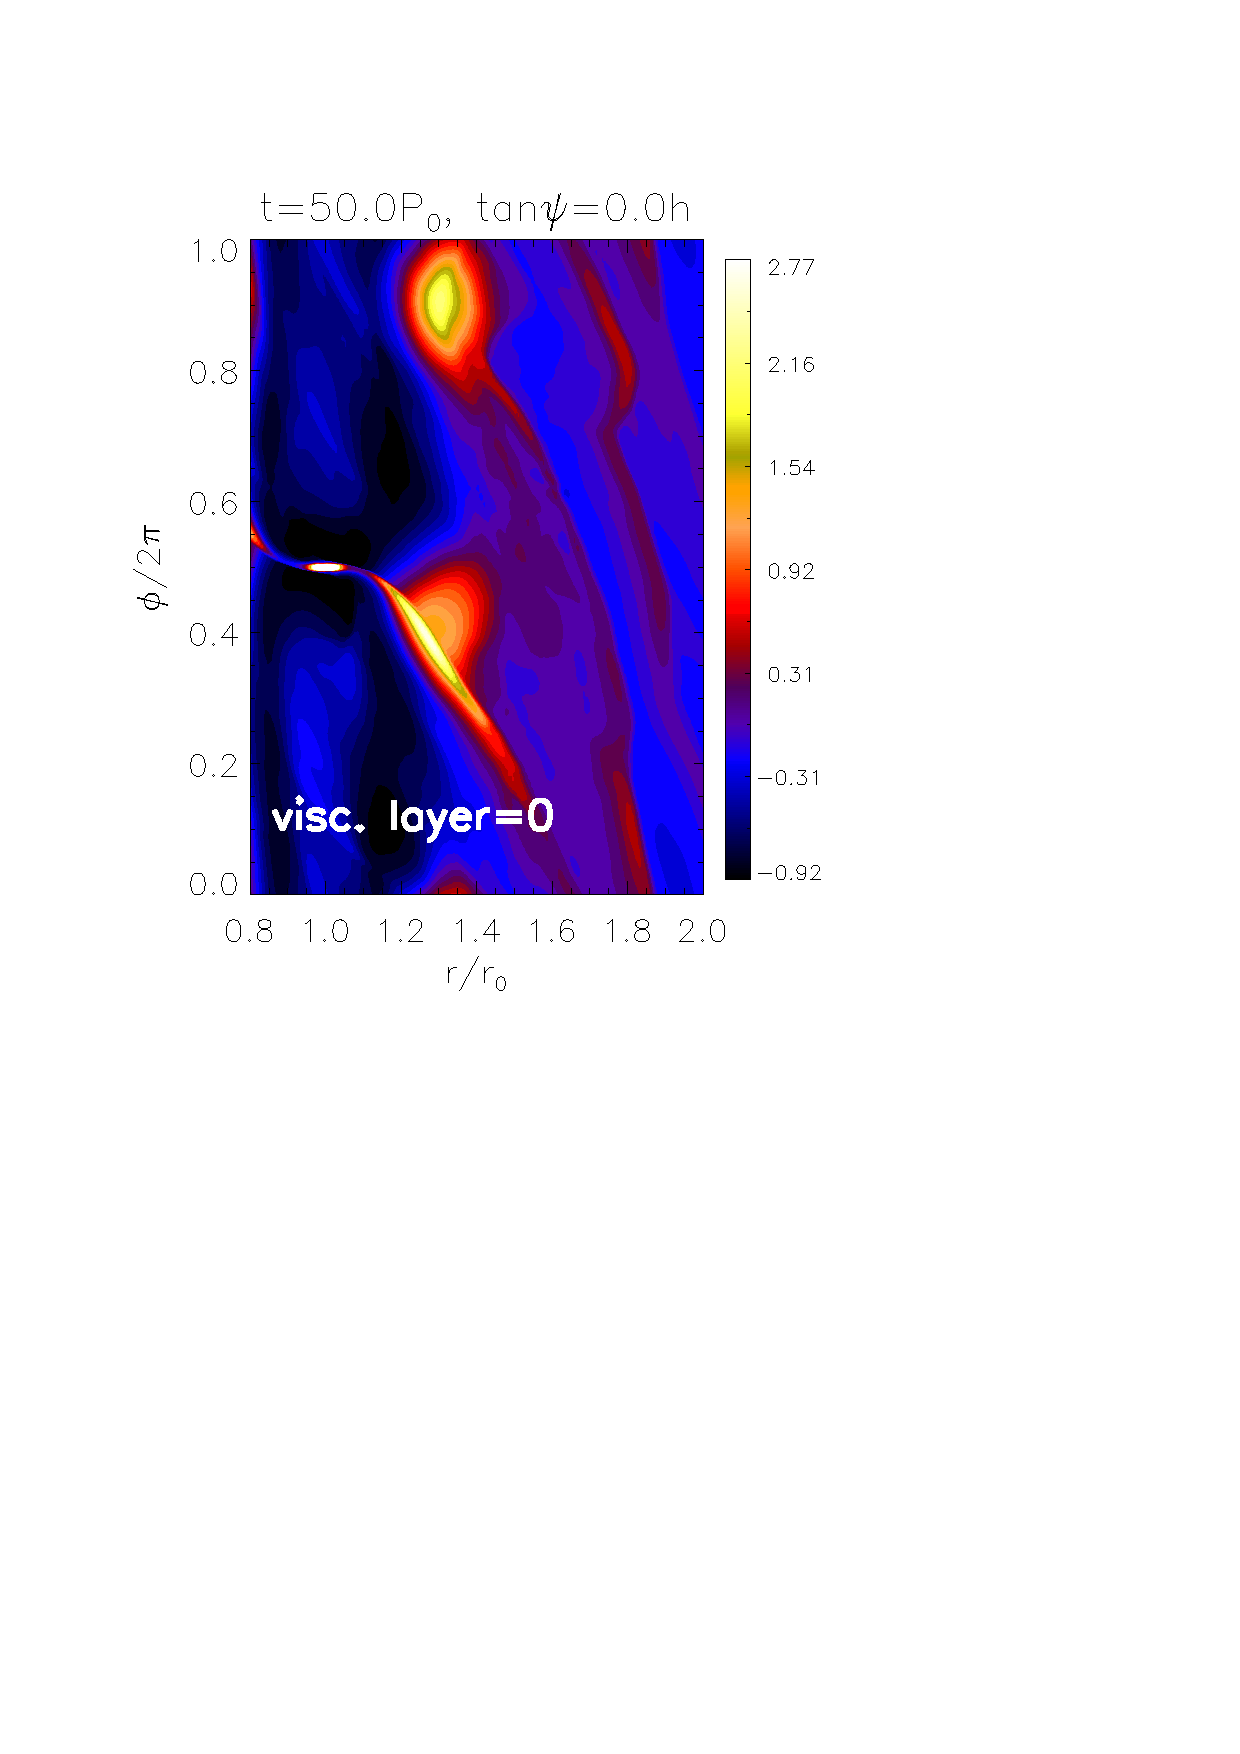
\includegraphics[scale=.43,clip=true,trim=0cm 1.84cm 0cm
     0cm]{figures/jup0_3h_pdisk_005}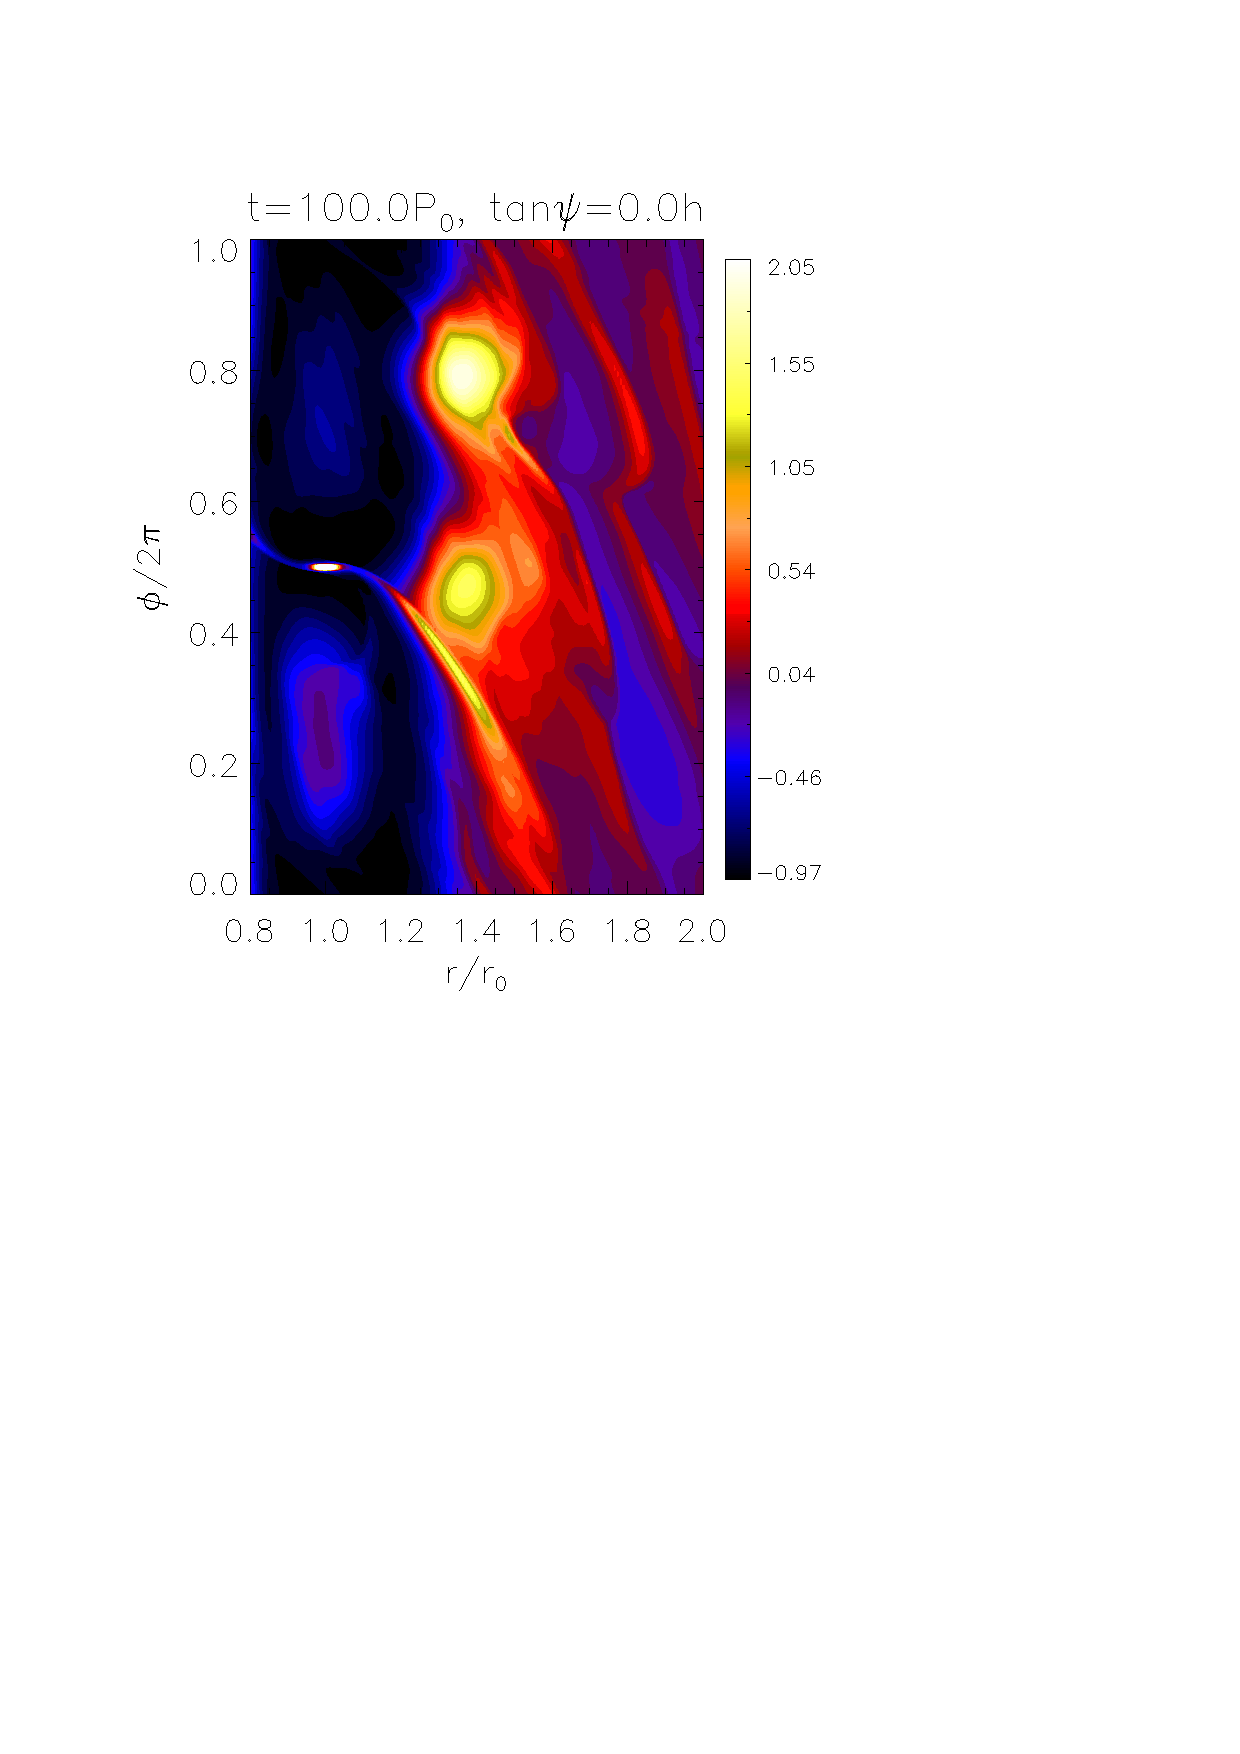
\includegraphics[scale=.43,clip=true,trim=2.3cm
     1.84cm 0cm 0cm]{figures/jup0_3h_pdisk_010}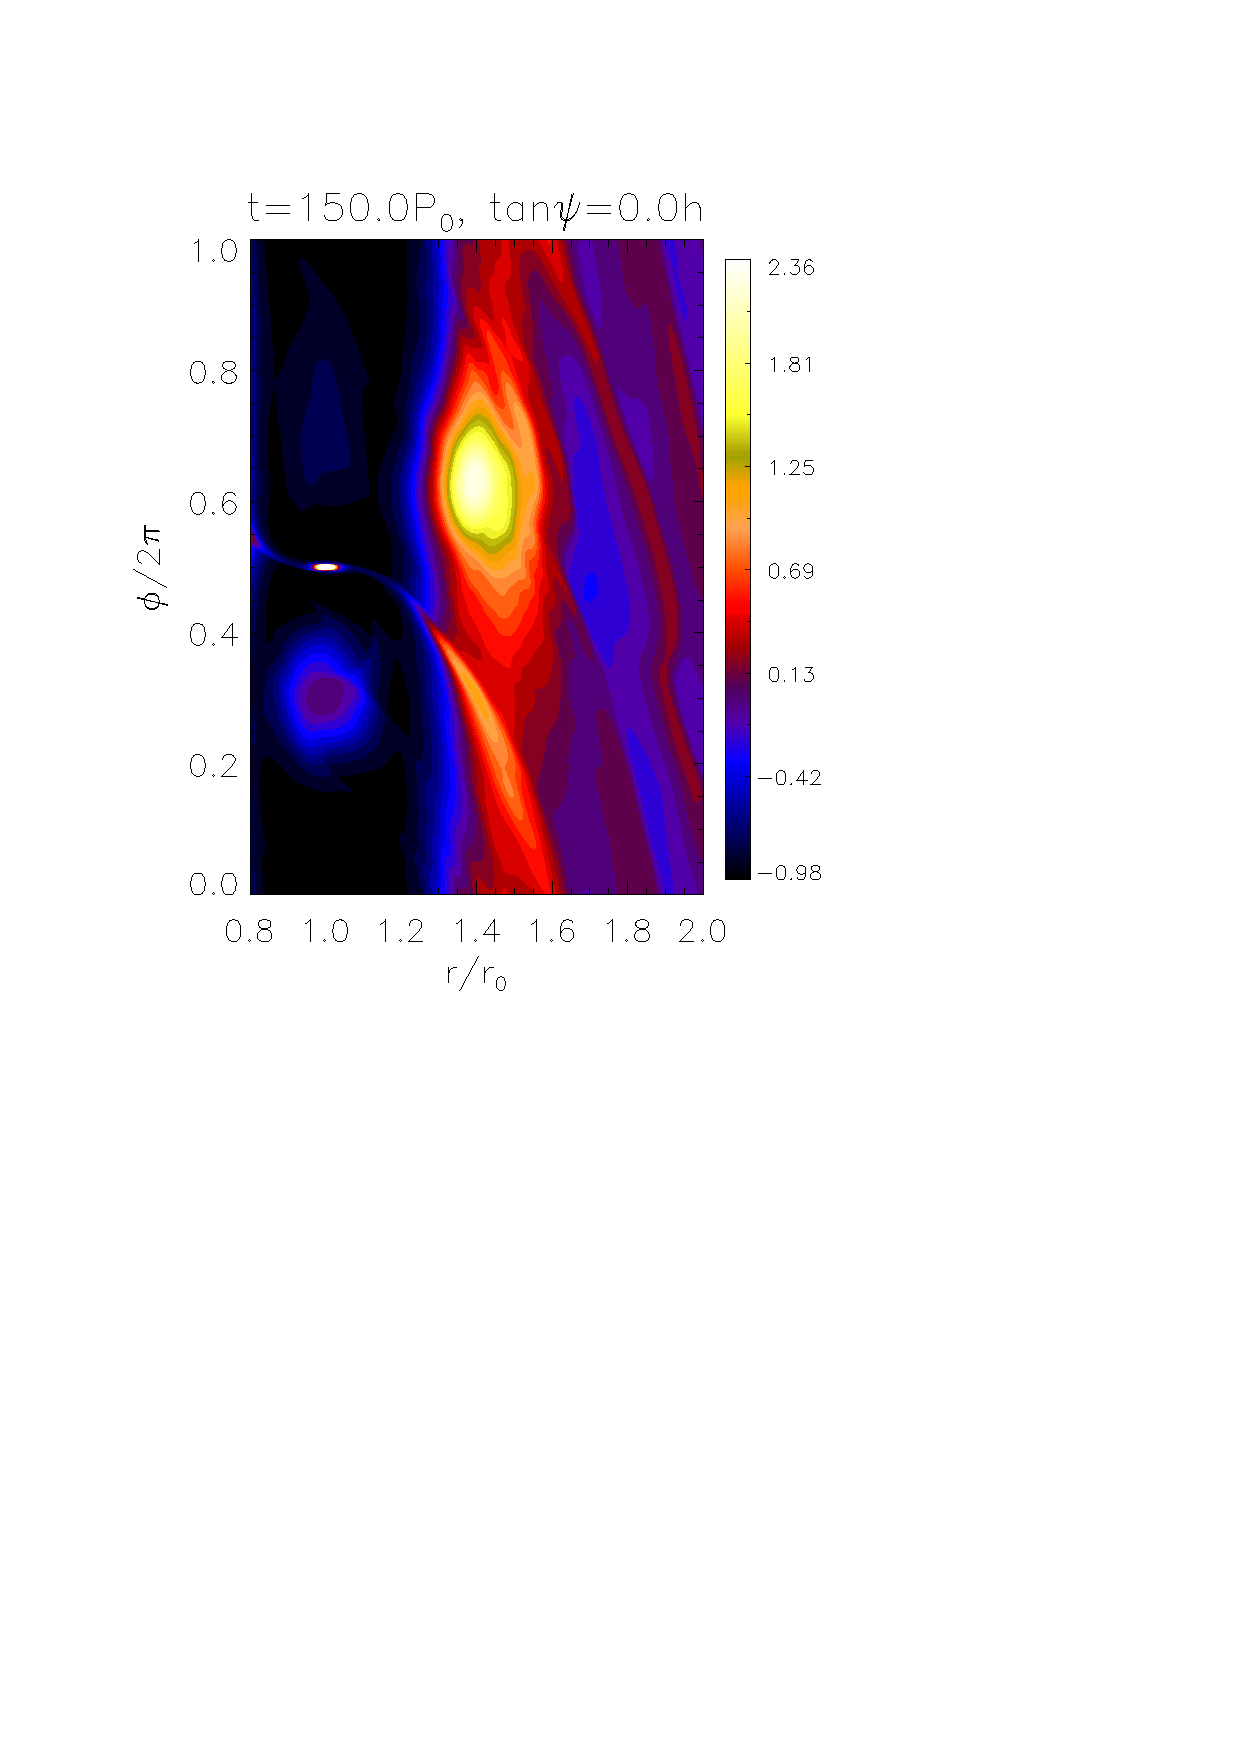
\includegraphics[scale=.43,clip=true,trim=2.3cm
     1.84cm 0cm 0cm]{figures/jup0_3h_pdisk_015}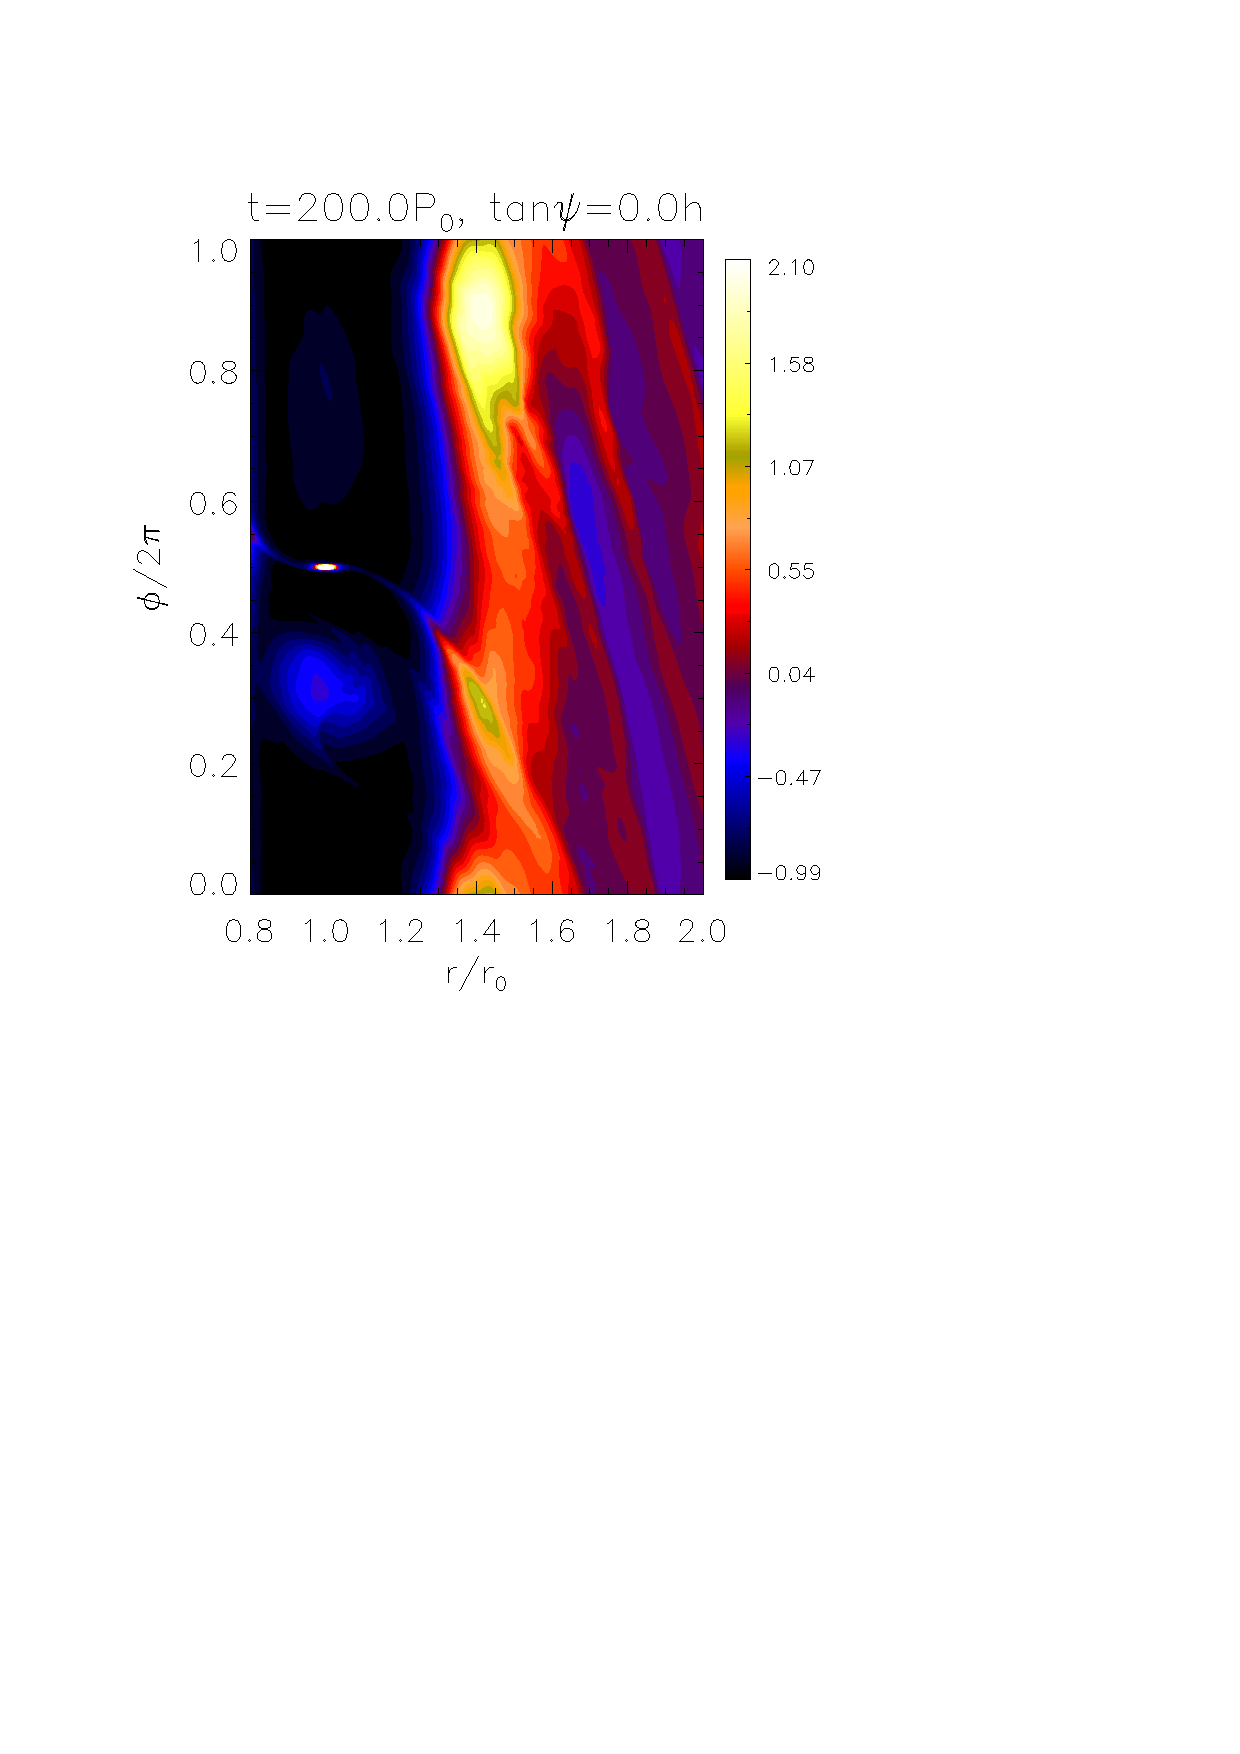
\includegraphics[scale=.43,clip=true,trim=2.3cm
     1.84cm 0cm 0cm]{figures/jup0_3h_pdisk_020}\\
    \includegraphics[scale=.43,clip=true,trim=0cm 1.84cm 0cm
     0.9cm]{figures/jup0d5_3h_pdisk_005.ps}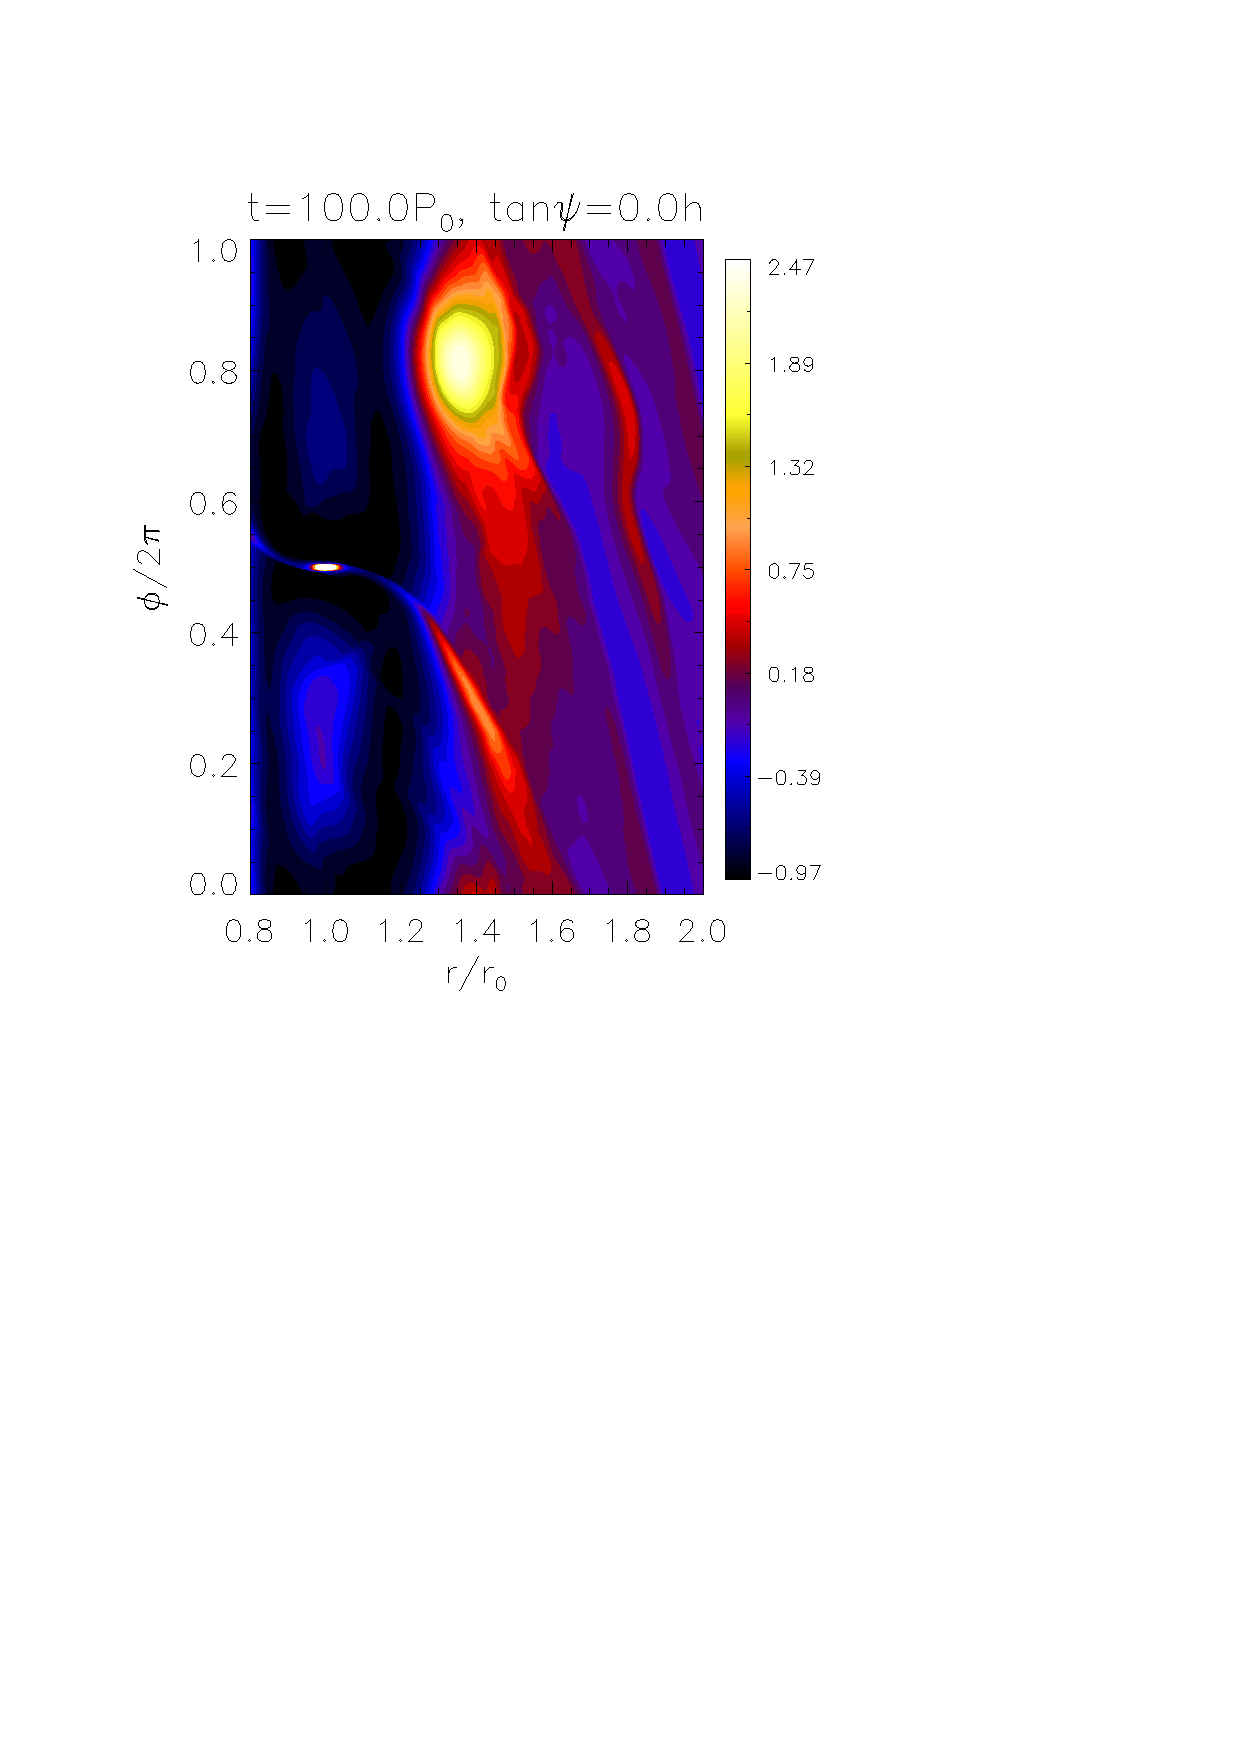
\includegraphics[scale=.43,clip=true,trim=2.3cm
     1.84cm 0cm 0.9cm]{figures/jup0d5_3h_pdisk_010}\\%\includegraphics[scale=.43,clip=true,trim=2.3cm
     %1.84cm 0cm 0cm]{figures/jup0.5_3h_pdisk_015}\includegraphics[scale=.43,clip=true,trim=2.3cm
     %1.84cm 0cm 0cm]{figures/jup0.5_3h_pdisk_020}\\
   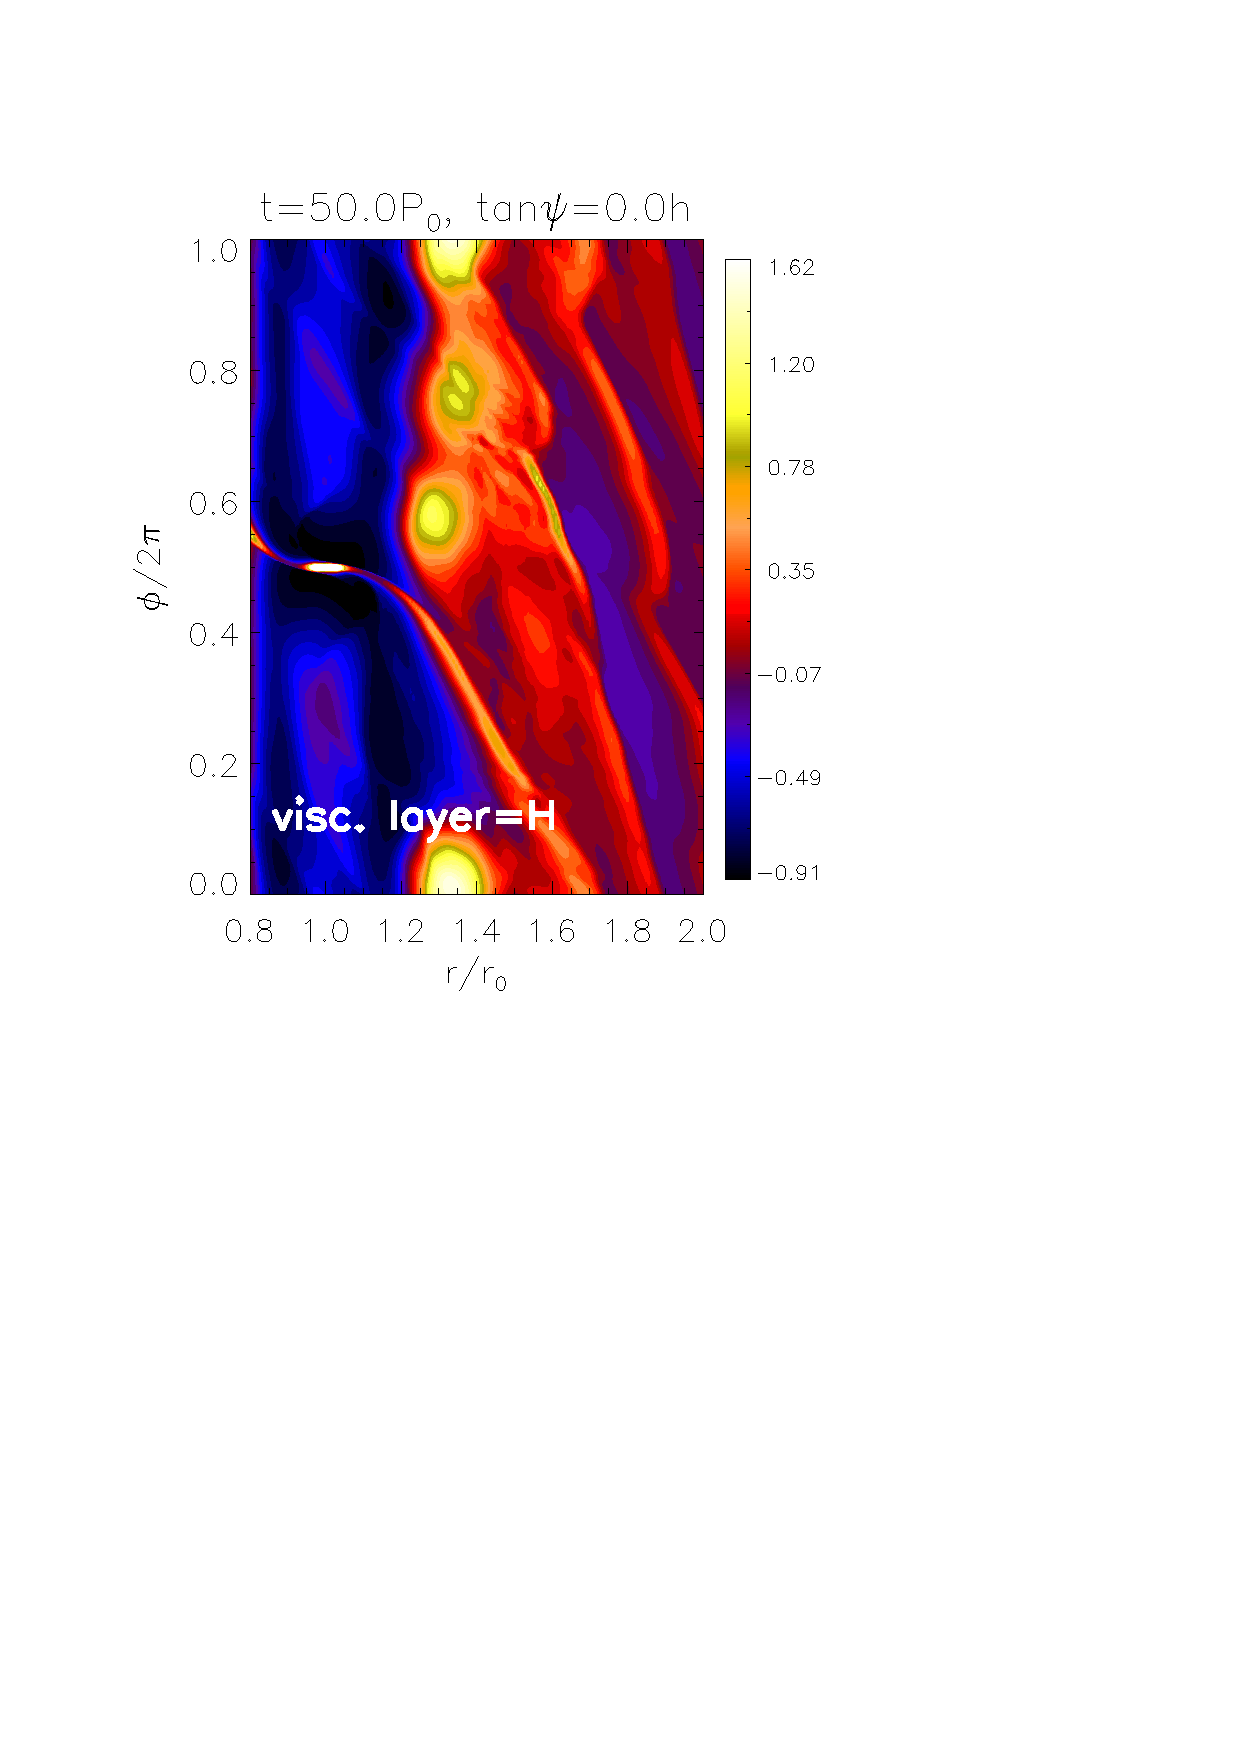
\includegraphics[scale=.43,clip=true,trim=0cm 0.cm 0.cm
     0.9cm]{figures/jup1_3h_pdisk_005}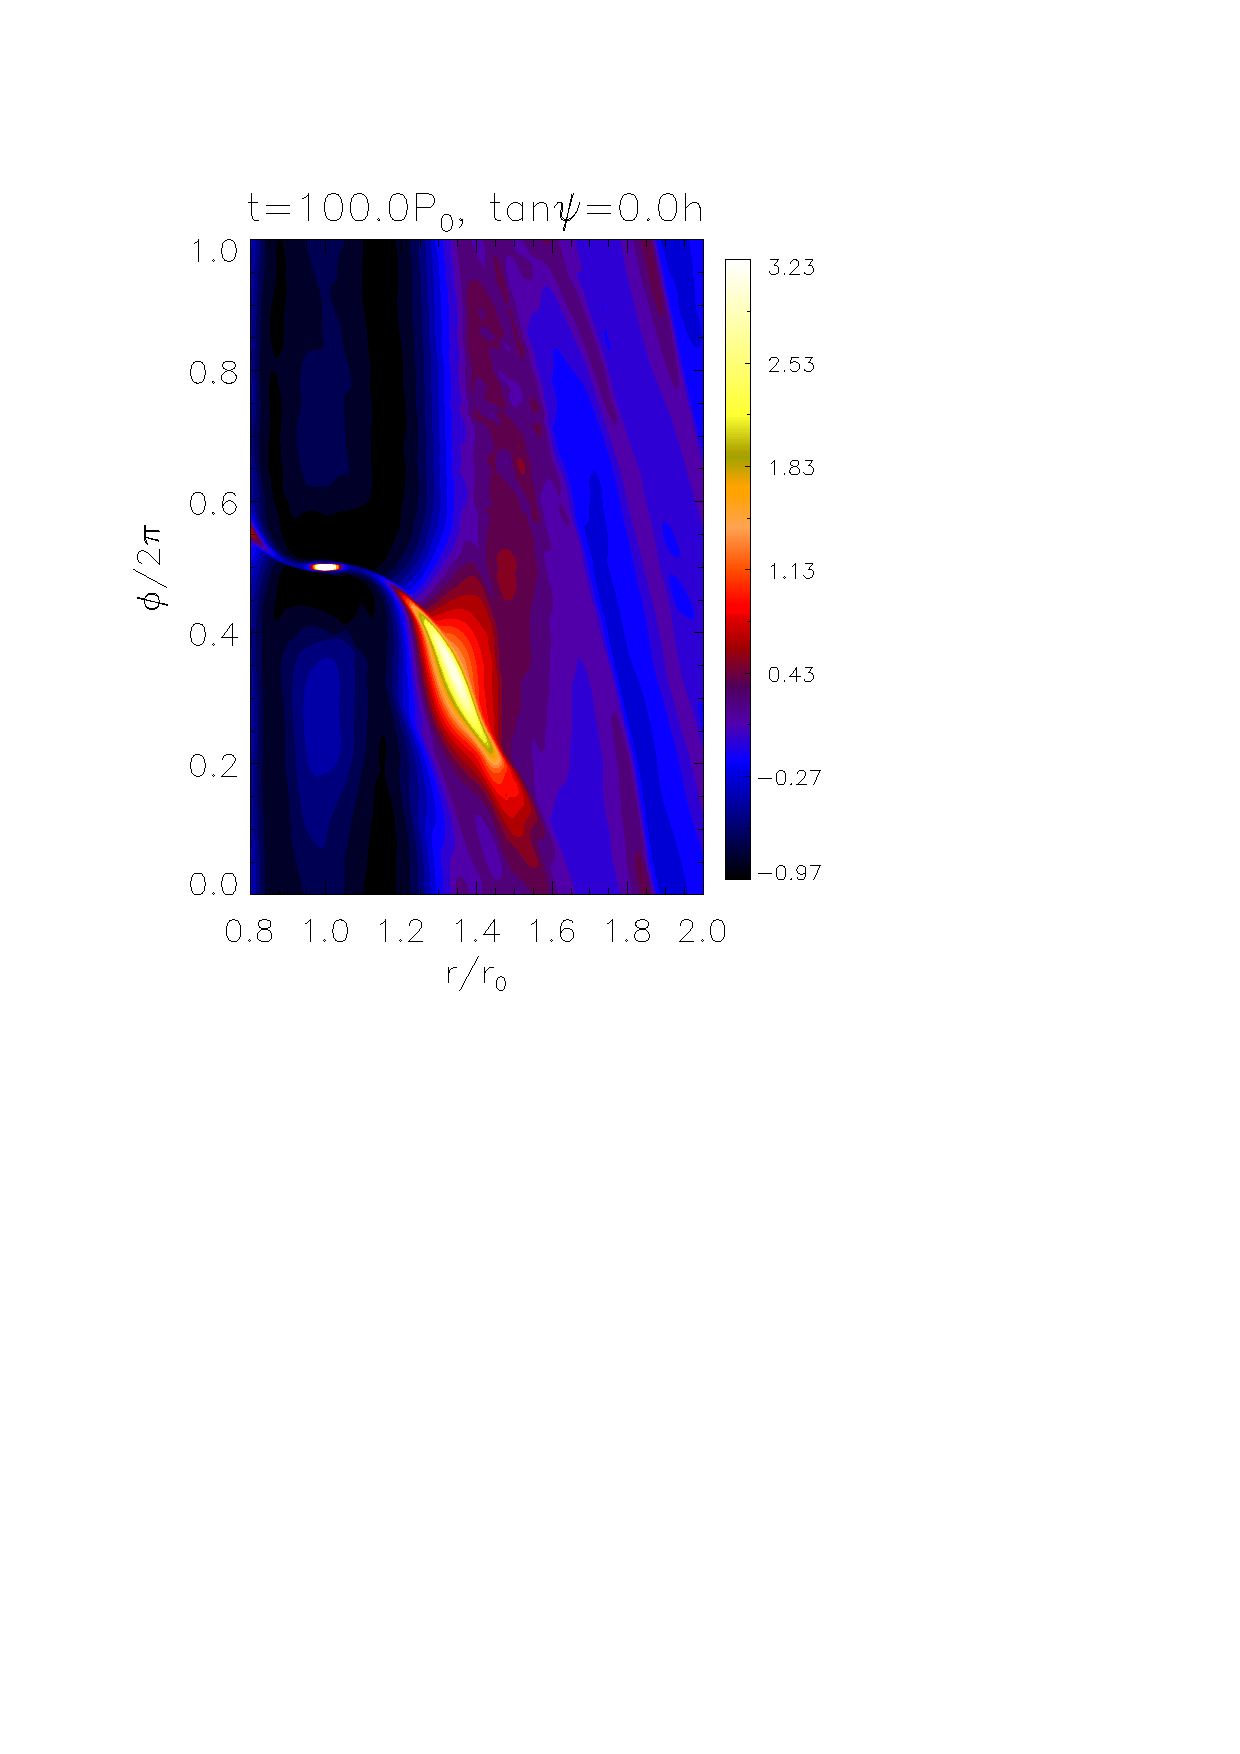
\includegraphics[scale=.43,clip=true,trim=2.3cm
     0.cm 0cm 0.9cm]{figures/jup1_3h_pdisk_010}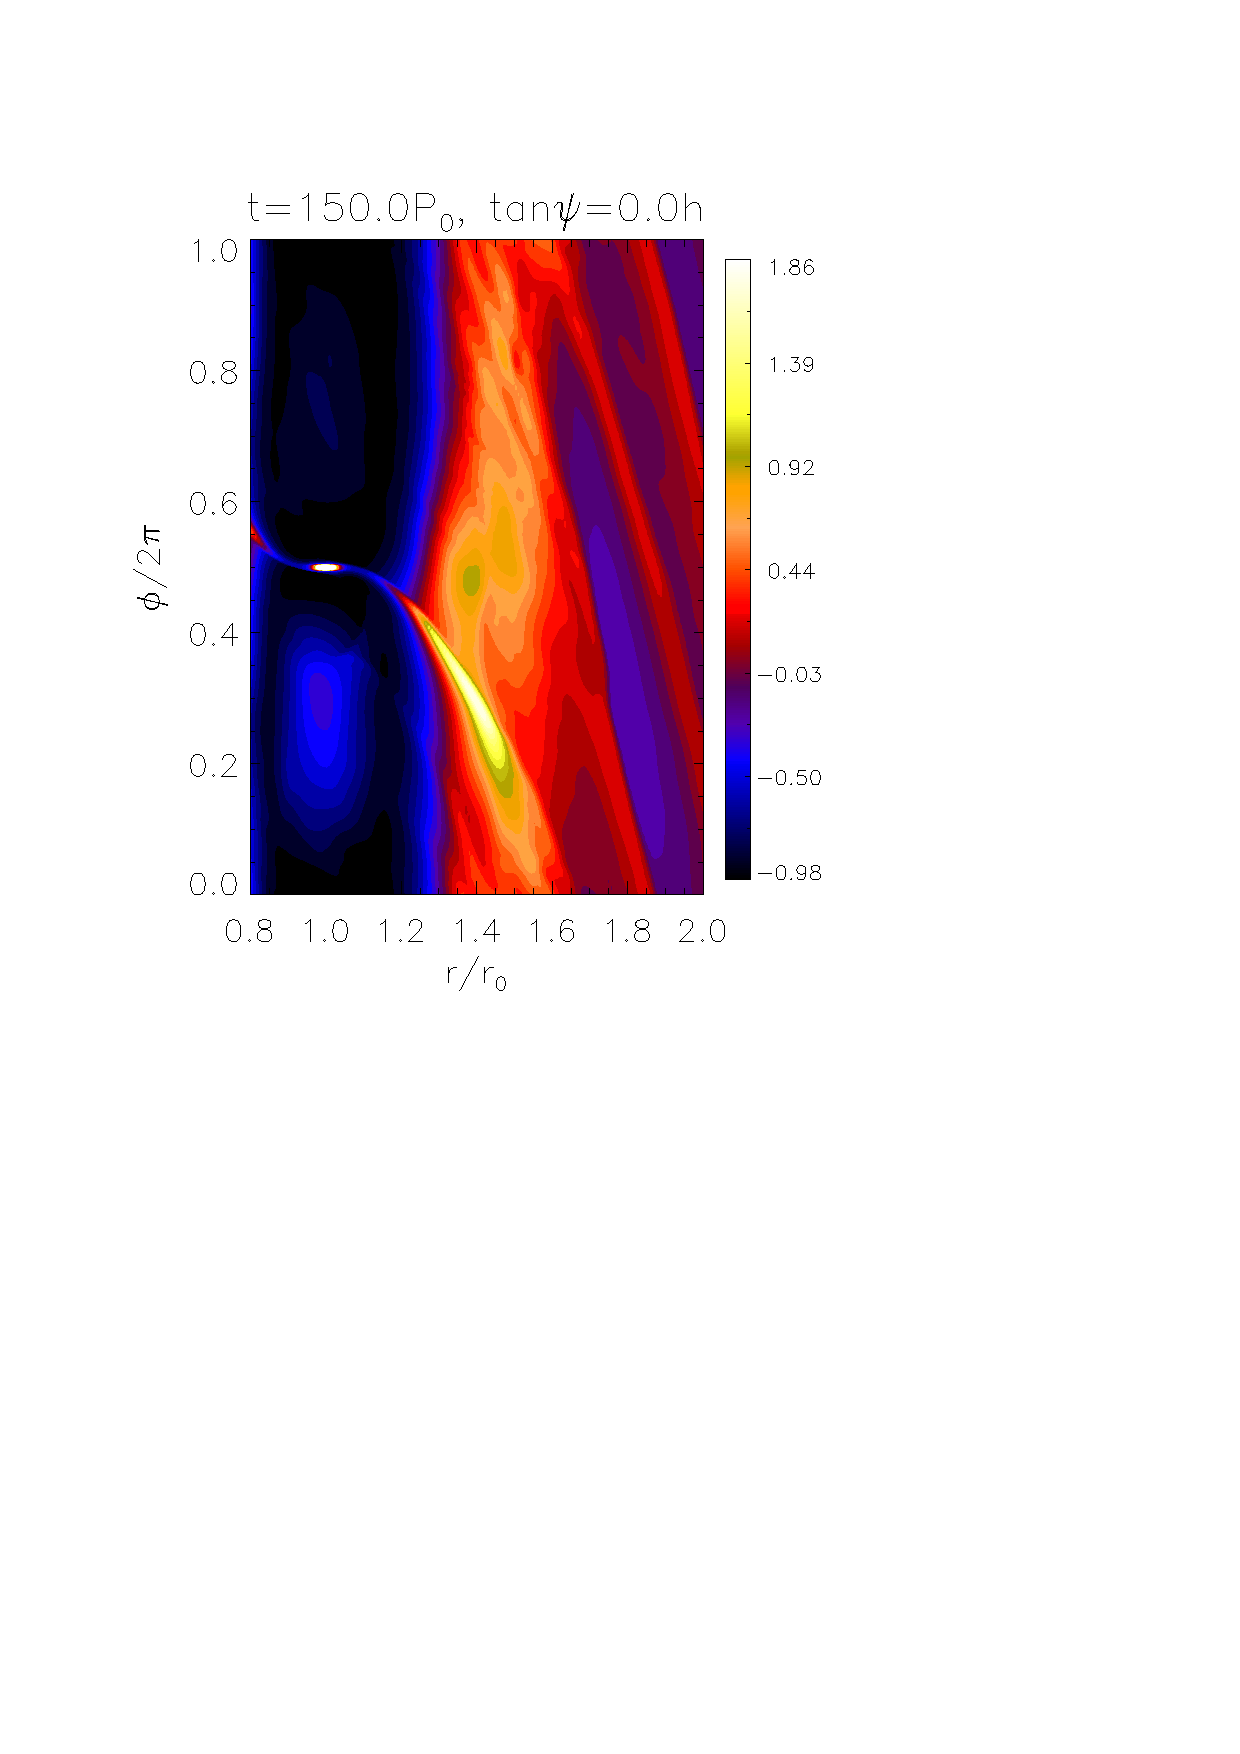
\includegraphics[scale=.43,clip=true,trim=2.3cm
     0.cm 0cm 0.9cm]{figures/jup1_3h_pdisk_015}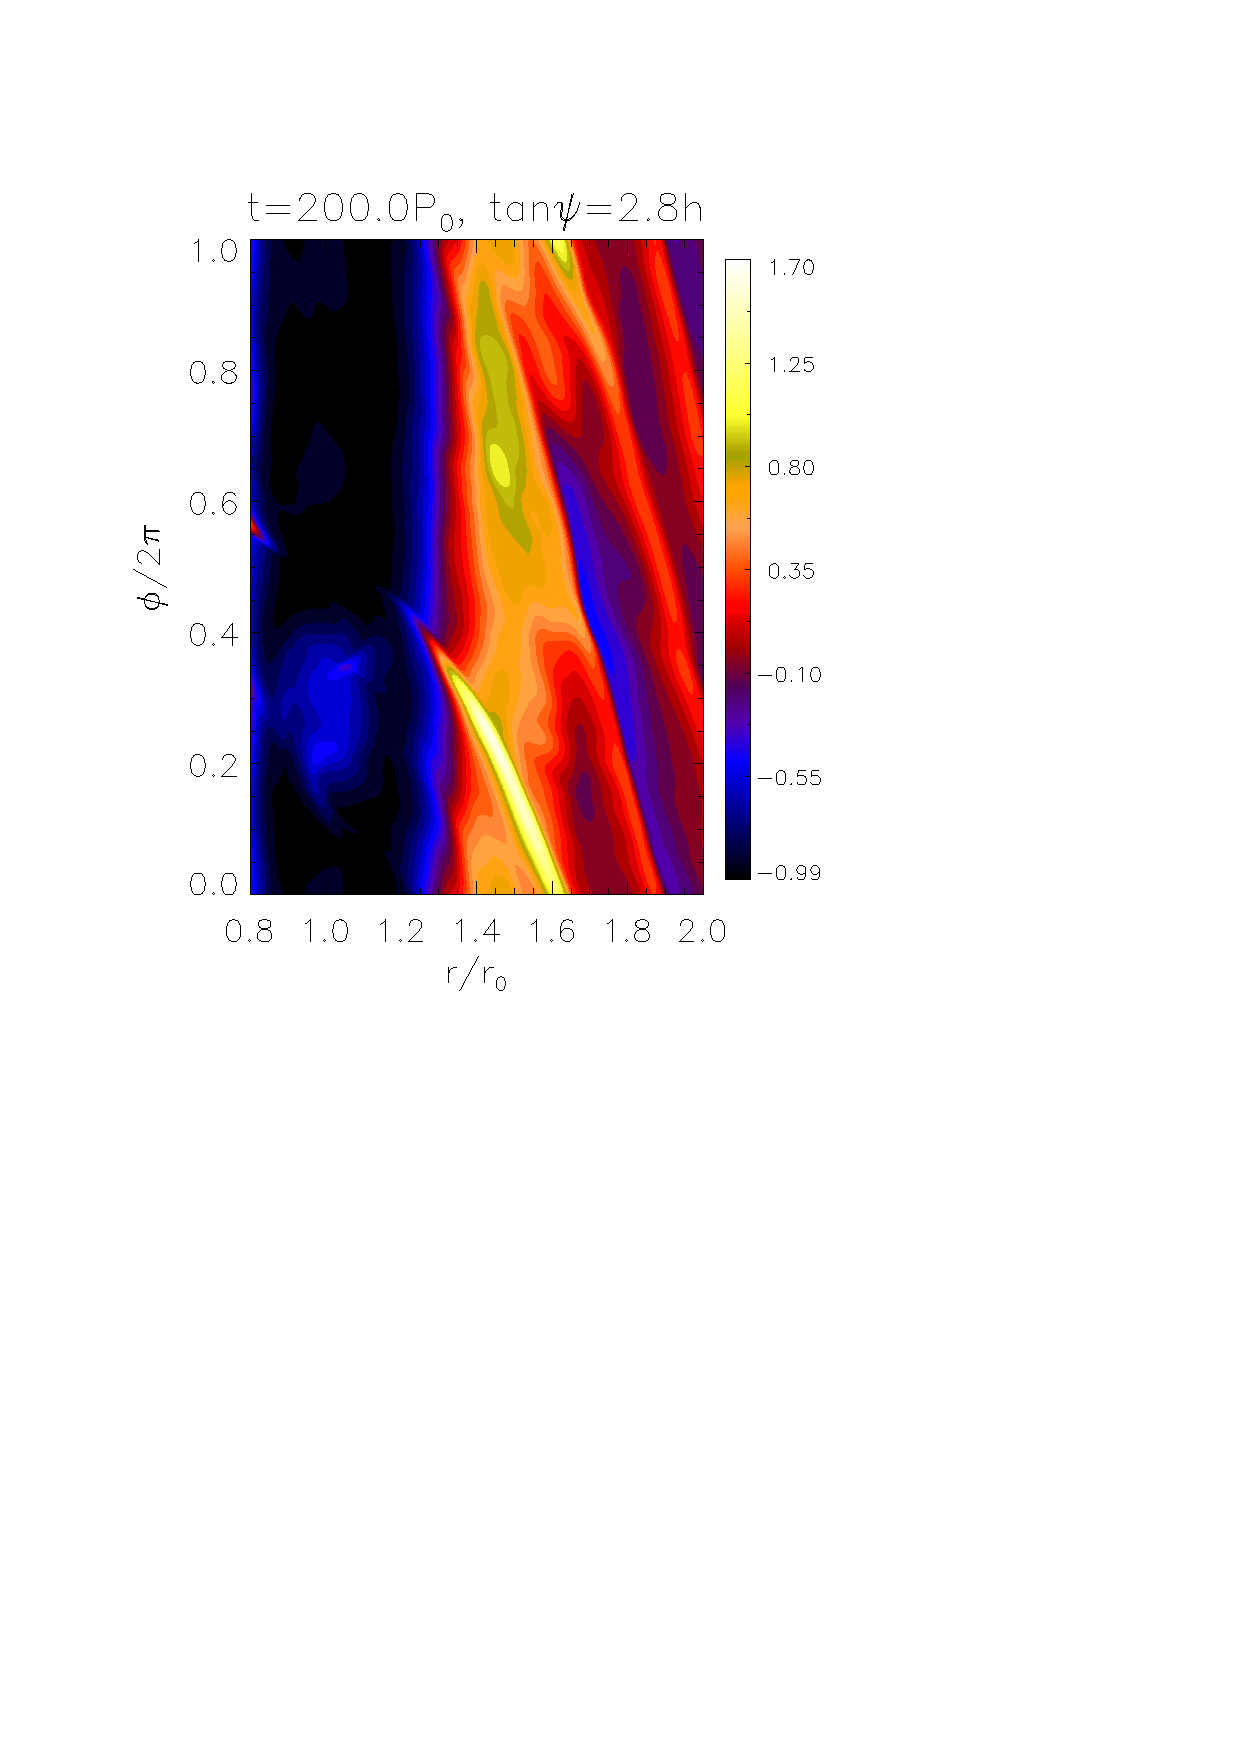
\includegraphics[scale=.43,clip=true,trim=2.3cm
     0.cm 0cm 0.9cm]{figures/jup1_3h_pdisk_020}\\
%    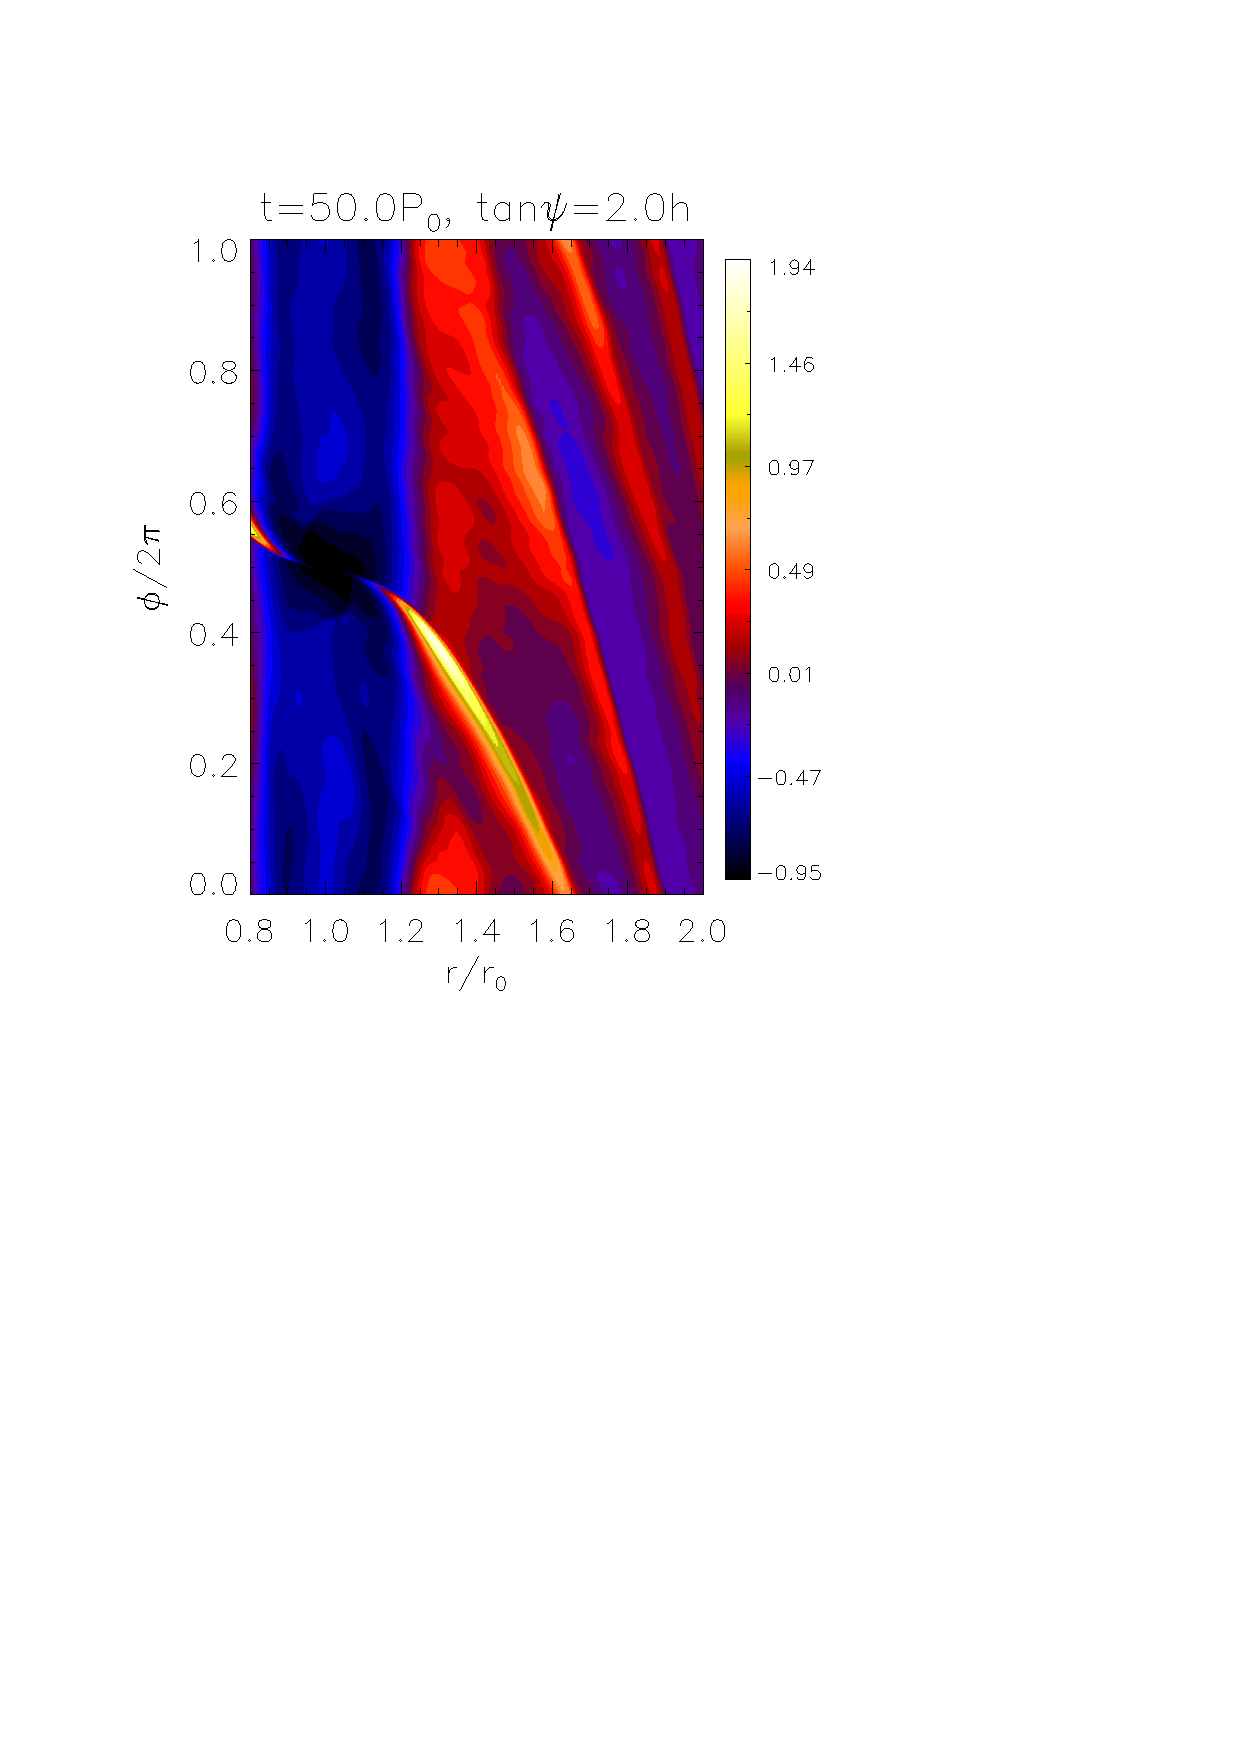
\includegraphics[scale=.43,clip=true,trim=0cm 0.cm 0.cm
%     0.9cm]{figures/jup2_3h_pdisk_005}
   \caption{Relative density perturbation $\Delta\rho$ for disc-planet
     simluations. The thickness of the viscous layer increases from
     top to bottom: case P0 (no viscous layer), case P0.5 (viscous
     layer of $0.5H$) and cases P1 (viscous layer of $H$). 
     \label{jup0_3h}}
\end{figure*}
 


%\subsection{Locally isothermal simulations}
